\documentclass[tikz, border=6pt]{standalone}
\IfFileExists{lmodern.sty}{\usepackage[T1]{fontenc}\usepackage{lmodern}}{}
\usepackage{amsmath,amssymb,bm}
\usetikzlibrary{arrows.meta}
\definecolor{Blue}{HTML}{3A76D8}
\definecolor{Ink}{HTML}{1F2937}
\definecolor{cF5B385}{HTML}{F5B385}
\definecolor{cEE9171}{HTML}{EE9171}
\definecolor{cE66E5E}{HTML}{E66E5E}
\definecolor{cDF4B4B}{HTML}{DF4B4B}
\begin{document}
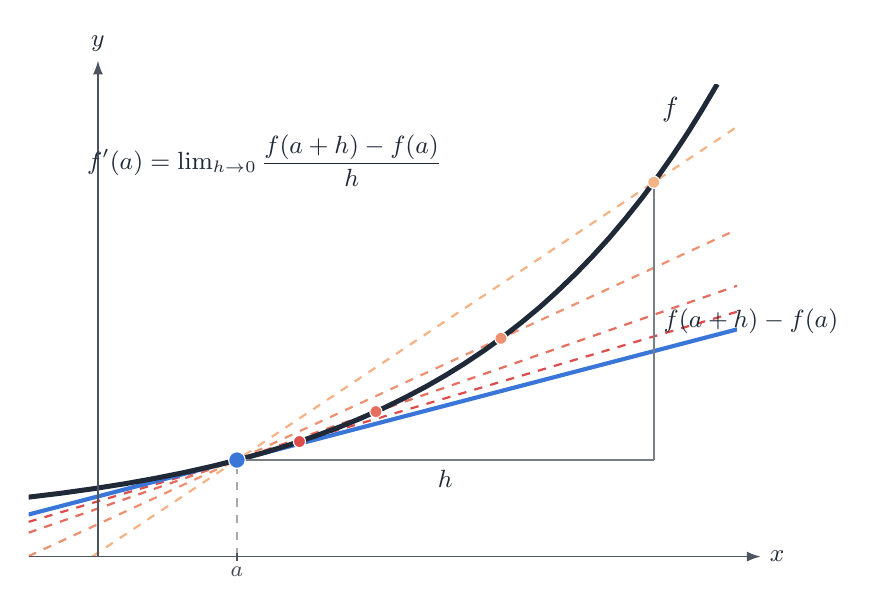
\begin{tikzpicture}[color=Ink, line width=0.5pt, >={Latex[length=5pt, width=3.6pt]}, line join=round]
  % axes ax1
  \begin{scope}
    \clip (0,0) rectangle (9,6);
    \draw[dashed, color=cF5B385, line width=0.8pt] (0.808,0) -- (9,5.46);
    \draw[dashed, color=cEE9171, line width=0.8pt] (0,0.005) -- (9,4.155);
    \draw[dashed, color=cE66E5E, line width=0.8pt] (0,0.303) -- (9,3.44);
    \draw[dashed, color=cDF4B4B, line width=0.8pt] (0,0.441) -- (9,3.11);
    \draw[color=Blue, line width=1.5pt] (0,0.534) -- (9,2.886);
    \draw[color=Ink, line width=1.8pt] (0,0.755) -- (0.421,0.806) -- (0.843,0.865) -- (1.234,0.927) --
        (1.625,0.997) -- (1.987,1.07) -- (2.348,1.151) -- (2.679,1.234) -- (3.01,1.326) -- (3.341,1.428)
        -- (3.642,1.531) -- (3.943,1.643) -- (4.214,1.754) -- (4.515,1.888) -- (4.786,2.021) --
        (5.057,2.164) -- (5.298,2.303) -- (5.538,2.452) -- (5.779,2.613) -- (6.02,2.787) --
        (6.261,2.974) -- (6.502,3.175) -- (6.712,3.365) -- (6.953,3.597) -- (7.164,3.815) --
        (7.375,4.047) -- (7.585,4.296) -- (7.796,4.561) -- (7.977,4.803) -- (8.187,5.102) --
        (8.368,5.375) -- (8.548,5.664) -- (8.747,6);
    \draw[color=Ink!40, dashed] (2.647,0) -- (2.647,1.226);
    \draw[color=Ink!60, line width=0.6pt] (2.647,1.226) -- (7.941,1.226);
    \draw[color=Ink!60, line width=0.6pt] (7.941,1.226) -- (7.941,4.754);
    \filldraw[fill=cF5B385, draw=white, line width=0.4pt] (7.941,4.754) circle[radius=2.2pt];
    \filldraw[fill=cEE9171, draw=white, line width=0.4pt] (6,2.772) circle[radius=2.2pt];
    \filldraw[fill=cE66E5E, draw=white, line width=0.4pt] (4.412,1.841) circle[radius=2.2pt];
    \filldraw[fill=cDF4B4B, draw=white, line width=0.4pt] (3.441,1.461) circle[radius=2.2pt];
    \filldraw[fill=Blue, draw=white, line width=0.4pt] (2.647,1.226) circle[radius=3pt];
  \end{scope}
  \draw[->, Ink!80, line width=0.6pt] (0,0) -- (9.3,0);
  \draw[->, Ink!80, line width=0.6pt] (0.882,0) -- (0.882,6.3);
  \draw[Ink!80, line width=0.5pt] (2.647,-0.05) -- (2.647,0.05);
  \node[anchor=north, font=\footnotesize, text=Ink!85, inner sep=2pt] (ax1-xt0) at (2.647,-0.05) {$a$};
  \node[anchor=north, font=\small] at (5.294,1.226) {$h$};
  \node[anchor=west, font=\small] at (7.941,2.99) {$f(a+h)-f(a)$};
  \node[anchor=south east] at (8.382,5.398) {$f$};
  \node[anchor=west, font=\small, align=center, inner sep=3pt] at (9.3,0) {$x$};
  \node[anchor=south, font=\small, align=center, inner sep=3pt] at (0.882,6.3) {$y$};
  \node[font=\small] at (3,5.0323) {$f'(a) = \lim_{h\to 0}\dfrac{f(a+h)-f(a)}{h}$};
\end{tikzpicture}
\end{document}
